\appendix
\section{DTR Algorithm}
\begin{algorithm}[ht!]
\caption{Deep Tabular Research}
\label{alg:dtr-framework}
\begin{algorithmic}[1]
\Require Query $q \in \mathcal{Q}$, Table $T \in \mathcal{T}$, Execution Environment $\mathcal{E}$, Learning Rate $\alpha$, Number of candidate paths $K$
\Ensure Answer $y \in \mathcal{Y}$

\State \textbf{// Step 1: Meta Operation Decomposition (MOD)}
\State Extract table metadata $\mathcal{T}_{meta}$ from $T$
\State $\mathcal{M}_q \gets$ MOD($q$, $\mathcal{T}_{meta}$) \Comment{Set of high-level meta operations}

\State \textbf{// Step 2: Candidate Macro Path Construction}
\State Initialize candidate path set $\Pi \gets \{\}$ 
\For{$k = 1$ to $K$}
    \State $\pi_k \gets$ generate\_candidate\_path($\mathcal{M}_q$) \Comment{Ordered sequence of meta operations}
    \State $\Pi \gets \Pi \cup \{\pi_k\}$
\EndFor

\State \textbf{// Step 3: Iterative Planning and Execution}
\While{not all paths executed or converged}
    \For{each path $\pi \in \Pi$}
        \State Compute expectation score $\mathbb{E}(\pi)$: 
        \[
        \mathbb{E}(\pi) = \hat{R}(\pi) + c \cdot P(\pi) \sqrt{\frac{\log \sum_{\pi'} N(\pi')}{1 + N(\pi)}}
        \]
    \EndFor
    \State Select top-ranked path(s) $\pi^*$ according to $\mathbb{E}(\pi)$
    \State $context \gets$ initial execution state in $\mathbb{E}$
    
    \For{each meta operation $m$ in $\pi^*$}
        \State $o, r \gets$ execute($m$, $context$, $\mathcal{E}$) \Comment{Execute and observe outcome and reward}
        \State Update Execution Experience Memory: $\mathcal{D} \gets \mathcal{D} \cup \{(m, context, o, r)\}$
        \State Update path reward:
        \[
        \hat{R}(\pi^*) \gets \frac{N(\pi^*) \hat{R}(\pi^*) + r}{N(\pi^*) + 1}, \quad N(\pi^*) \gets N(\pi^*) + 1
        \]
        \If{execution failed or outcome invalid}
            \State Replan: $\pi^* \gets$ Macro Path Planner($\mathcal{M}_q$, $\mathcal{D}$)
            \State break \Comment{Restart path execution with revised plan}
        \EndIf
        \State Update $context$ according to $o$
    \EndFor
\EndWhile

\State \textbf{// Step 4: Return final answer}
\State $y \gets$ extract\_answer($\pi^*$, $\mathcal{D}$)
\State \Return $y$
\end{algorithmic}
\end{algorithm}


\section{DTR-Bench Dataset Curation}
We introduce \textbf{DTR-Bench} (Deep Tabular Research Benchmark), a specialized benchmark for evaluating deep analytical reasoning capabilities over tabular data. Unlike existing table QA benchmarks that focus on simple fact retrieval or single-step reasoning, DTR-Bench emphasizes complex statistical analysis tasks that reflect real-world data science workflows. The benchmark comprises \textbf{500 scenario-driven question-answer pairs} from diverse domains, each requiring sophisticated analytical reasoning such as correlation analysis, inequality measurement, anomaly detection, and statistical hypothesis testing. 
This benchmark is derived from a curated selection of Excel spreadsheets sourced from RealHitBench, encompassing various domains including Economy, Business, and Education.

\subsection{Scenario-Driven Question Generation}
\label{sec:question_generation}

A key innovation of DTR-Bench is the \textbf{scenario-driven question generation} approach. Each question is grounded in a realistic user persona with domain-specific analytical needs, ensuring that questions reflect authentic data science tasks rather than artificial academic exercises.

\paragraph{User Persona Design}
\label{sec:personas}

We define 8 distinct user personas, each representing a real-world role that regularly performs deep tabular analysis:

\begin{table}[h]
\centering
\caption{User Persona Distribution in DTR-Bench}
\label{tab:persona_distribution}
\resizebox{\textwidth}{!}{%
\begin{tabular}{lrl}
\toprule
\textbf{User Persona} & \textbf{\ Questions} & \textbf{Primary Analysis Focus} \\
\midrule
Social Researcher & 105 & Inequality analysis (Gini coefficient, Lorenz curves), demographic patterns \\
Student/Researcher & 88 & Statistical hypothesis testing (ANOVA), effect size calculation (Cohen's $d$, $\eta^2$) \\
Government Staff & 62 & Longitudinal policy impact assessment, equity-efficiency trade-offs \\
Data Analyst & 61 & Dimensionality reduction, cohort analysis, z-score-based anomaly detection \\
Business Owner & 55 & Profitability decomposition, BCG matrix classification, break-even analysis \\
Procurement Manager & 53 & Supplier concentration (HHI), risk-performance matrices \\
Sales Manager & 40 & Multi-dimensional performance analysis, trend detection \\
Investor & 36 & Risk-return analysis, efficient frontier identification, valuation ratios \\
\bottomrule
\end{tabular}%
}
\end{table}

\paragraph{Question Template Design}
Each persona has 4 specialized question templates requiring analytical reasoning. Templates are mainly designed to: a. \textbf{Reference specific columns} using quoted identifiers (e.g., \texttt{"Revenue"})
b. \textbf{Specify analytical methods} (correlation, ANOVA, Gini coefficient, HHI, etc.) c.  \textbf{Request structured outputs} (rankings, statistical measures, interpretations). Table~\ref{tab:persona-templates} illustrates representative question templates for each persona type.

\begin{table}[htbp]
\centering
\caption{Representative Question Templates by Persona}
\label{tab:persona-templates}
\small
% 关键修改：添加这一行，将表格宽度拉伸至文本宽度
\resizebox{\textwidth}{!}{%
\begin{tabular}{@{}p{2.8cm}p{2.8cm}p{10cm}@{}}
\toprule
\textbf{Persona} & \textbf{Analysis Type} & \textbf{Template Example} \\
\midrule
Investor & Risk-Return Analysis & 
Conduct a risk-return analysis across all \texttt{\{Category\}} by examining the relationship between \texttt{\{NumericCol1\}} (returns) and \texttt{\{NumericCol2\}} (risk metrics). Identify the efficient frontier segments. \\
\addlinespace[3pt]
Social Researcher & Inequality Analysis & 
Measure the distribution of \texttt{\{NumericCol\}} across \texttt{\{Category\}} using Gini coefficient and decile ratios. Investigate structural factors driving inequality. \\
\addlinespace[3pt]
Data Analyst & Anomaly Detection & 
Use statistical methods (z-scores) to identify unusual patterns in \texttt{\{NumericCol\}} across \texttt{\{Category\}}. Investigate anomalies and assess impact. \\
\addlinespace[3pt]
Student/Researcher & Statistical Testing & 
Conduct rigorous statistical analysis of \texttt{\{NumericCol\}} across \texttt{\{Category\}}: test for normality, perform ANOVA/Kruskal-Wallis tests, and calculate effect sizes. \\
\bottomrule
\end{tabular}
} % 注意：这里要闭合 resizebox
\end{table}

% \begin{table}[h]
% \centering
% \caption{Supported Statistical Analysis Methods}
% \label{tab:analysis_methods}
% \resizebox{\textwidth}{!}{%
% \begin{tabular}{lll}
% \toprule
% \textbf{Analysis Handler} & \textbf{Statistical Methods} & \textbf{Output Components} \\
% \midrule
% \texttt{correlation} & Pearson correlation & Overall $r$, per-category $r$, sample sizes \\
% \texttt{trend} & Linear regression & Slope, residual-based anomalies (z-scores) \\
% \texttt{inequality} & Gini coefficient & Gini value, top/bottom decile shares, ranked categories \\
% \texttt{group\_difference} & One-way ANOVA & $F$-statistic, $\eta^2$, Cohen's $d$, group summary stats \\
% \texttt{anomaly\_detection} & Z-score, IQR rule & High/low outliers, threshold values \\
% \texttt{concentration} & Herfindahl-Hirschman Index & HHI, top-1/3/5 shares, ranked contributors \\
% \texttt{bcg\_matrix} & Quadrant classification & Stars, Cash Cows, Question Marks, Dogs \\
% \texttt{ratio\_ranking} & Division, aggregation & Top/bottom categories by ratio \\
% \texttt{growth\_proxy} & Period comparison & Delta, percentage change, ranked growth \\
% \texttt{decomposition} & Contribution analysis & Category shares, correlation, top drivers \\
% \bottomrule
% \end{tabular}%
% }
% \end{table}

\subsection{Quality Assurance}
\label{sec:quality}
To ensure benchmark quality, we implement multiple validation steps:
\begin{itemize}
    \setlength{\itemsep}{0pt}
    \setlength{\parskip}{0pt}
    \setlength{\parsep}{0pt}
    \item \textbf{Column Validity Filtering}: Columns with invalid names (e.g., ``Unnamed:'', purely numeric headers, CJK characters) are excluded
    \item \textbf{Template-Table Compatibility}: Templates requiring specific column types (numeric, categorical, temporal) are only instantiated when suitable columns exist
    \item \textbf{Time-Series Validation}: Templates involving trend analysis are skipped for tables without detectable temporal columns
    \item \textbf{Duplicate Prevention}: Questions are deduplicated using normalized string comparison
    \item \textbf{Answer Verification}: All reference answers are computed programmatically from actual table data, ensuring reproducibility
\end{itemize}

\paragraph{Answer Key Points (KeyPoints) for Evaluation}
\label{sec:keypoints}
In addition to validating that reference answers are computed from the underlying table data, we attach an \texttt{AnswerKeyPoints} field to each instance as explicit, machine-checkable grading criteria. This enables fine-grained evaluation (e.g., key-point coverage) beyond string matching.

\begin{figure}[h]
\begin{tcolorbox}[
    colback=gray!5,
    colframe=gray!60,
    fonttitle=\bfseries,
    boxrule=0.5pt
]
\textbf{Answer:} \\
    Gini coefficient of total Revenue across Region: 0.342... \\
\textbf{AnswerKeyPoints:} \\
    "Aggregate the numeric metric by category.", \\
    "Compute an inequality metric such as the Gini coefficient.", \\
    "Report concentration (e.g., top vs bottom shares) and top categories."
\end{tcolorbox}
\end{figure}



\section{Implementation Details}\label{implement}
\subsection{Benchmark Datasets}
\label{sec:datasets}

\paragraph{DTR-Bench: Long-Horizon Analytical Queries.}
To profoundly evaluate the performance for complex and long-horizon tabular reasoning datasets, we construct an additional DTR-Bench based on tables in RealHitBench. Using table meta information and expert-designed templates combined with \texttt{DeepSeek-3.2}, we generate 500 long-form analytical queries that require multi-step reasoning and execution. These queries span five categories: \textit{Analysis}: multi-stage aggregation and interpretation. \textit{Visualization}: chart generation and visual comparison. \textit{Calculation}: chained numerical computation. \textit{Comparison}: cross-group or temporal comparison. \textit{Conditional Calculation}: conditional aggregation and filtering.

Each query typically requires planning over multiple operations and intermediate execution states, making them unsuitable for shallow or single-pass reasoning approaches.

For the evaluation, we report two following metrics. \textit{Win Rate}: proportion of instances where a model outperforms baselines (ties counted as $0$). \textit{Score Rate}: proportion of instances where a model is not worse than baselines (ties counted as $0.5$).


\paragraph{RealHitBench.}
We adopt RealHitBench~\cite{wu2025realhitbench} as our primary benchmark, a large-scale dataset designed for evaluating reasoning over real-world, unstructured tables.
RealHitBench contains tables with heterogeneous layouts, including merged cells, bidirectional and hierarchical headers, missing values, and implicit semantic regions.
The benchmark categorizes tasks into multiple reasoning types and provides fine-grained evaluation protocols.

We evaluate DTR on the following RealHitBench task categories: \textit{Fact Checking}: verifying factual statements grounded in table entries. \textit{Numerical Reasoning}: performing arithmetic and aggregation over table values. \textit{Structure Comprehension}: understanding table organization, header hierarchy, and alignment. \textit{Data Analysis}: multi-step analytical reasoning requiring aggregation, comparison, and synthesis. \textit{Visualization}: generating charts or structured visual outputs based on tabular data.


For Fact Checking, Numerical Reasoning, and Structure Comprehension, we report \textit{Exact Match (EM)} and \textit{F1} scores following the benchmark protocol.
Data Analysis tasks are evaluated using \textit{LLM-based evaluation} and \textit{ROUGE} metrics to assess semantic correctness and completeness.
Visualization tasks are evaluated using \textit{Execution Correctness Rate (ECR)} and \textit{Pass@1}, measuring whether the generated visualization code executes successfully and produces the expected output.


\subsection{Baselines}
\label{sec:baselines}

We compare DTR against a diverse set of baselines spanning table-specialized models, general-purpose large language models, and agent-based reasoning frameworks~\cite{zheng2024multimodal, lu2025youtu}. 
\textbf{Table-specific Models.} TableGPT~\cite{gong2020tablegpt}: a representative table-focused language model designed for structured table question answering. \textbf{General-purpose LLMs.} DeepSeek-3.2: a strong open-source large language model with competitive reasoning capabilities; \textbf{Agentic Frameworks.} ST-RAPTOR~\cite{tang2025st}: a retrieval-augmented agent framework for structured reasoning; Tree Thinker~\cite{wu2025realhitbench}: a tree-based reasoning agent that explores multiple reasoning branches; \textbf{CodeLoop}: we craft a straightforward execution-centric agentic framework that iteratively generates and debugs code. All baselines are evaluated under comparable settings, with access to the same table inputs and query information.
Unless otherwise specified, we use publicly released model checkpoints and default decoding configurations. The base LLMs we adopted is Qwen3 1.7B\&4B~\cite{yang2025qwen3} and DeepSeek V3~\cite{liu2024deepseek}.

\section{Related Work}
\subsection{Deep Research and Agentic Reasoning}
Recent advances in large language models have aroused growing interest in agentic systems that perform multi-step reasoning through interaction with external tools, environments, or intermediate states~\cite{zhao2024expel,huang2024understanding,gong2020tablegpt}. A line of deep research work often focuses on long-horizon problem solving, where models iteratively plan and revise their strategies based on intermediate feedback~\cite{wolflein2025llm}. Typical examples include agents augmented with external tools, systems that separate planning from execution, and methods that rely on self-reflection or self-correction across multiple steps~\cite{renze2024self,dagan2023dynamic}. Notably, many existing agent-based approaches emphasis on language-level planning and reasoning~\cite{ge2025samule,song2023llm}. While such approaches have demonstrated strong performance on structured benchmarks, they typically assume reliable intermediate steps and make limited use of execution feedback. In contrast, our work treats deep search as a continual process, where accumulated action experience guides path selection and enables more robust behavior.

\subsection{Tabular Reasoning and Table Question Answering}

Tabular reasoning has been extensively studied in the context of table question answering, semantic parsing, and data analysis~\cite{zhao2023openrt}. Early approaches typically focused on mapping natural language queries to logical forms or executable programs over well-structured tables with clean schemas and regular layouts~\cite{akhtar2023exploring,Perzina2014MicrosoftEA}. Recent methods leverage large language models to perform tabular reasoning in a more flexible manner through straightforwardly interpreting table contents. Such pipelines reason over tables using code generation, textual serialization, or prompting strategies~\cite{wang2024chain,Zhu2024AutoTQATA,Shi2024EHRAgentCE}. Existing work on tabular reasoning spans a diverse set of tasks, including fact checking, numerical reasoning, data analysis, and table-based visualization~\cite{Wu2024TableBenchAC}, where models are required to interpret structured or semi-structured information and perform reasoning over rows, columns, and cell values~\cite{Sun2024ASO}. Despite substantial progress, chain-of-thought prompting and single-pass code generation can be sensitive to early reasoning decisions in complex tabular analysis. While hybrid symbolic approaches improve robustness, they lack mechanisms for iterative decision making with accumulated experience~\cite{kulkarni2025llmsymbolicintegrationrobusttemporal}. 

Our work bridges this gap by introducing a unified framework for Deep Tabular Research that integrates operator-level execution with continual experience-driven decision making. By explicitly modeling path selection, execution, and memory as interacting components, the proposed approach extends prior reasoning systems to handle complex, unstructured tables requiring iterative analysis and revision.


% Chain-of-Thought prompting and single-pass program generation have been shown to be brittle in these settings, as early reasoning errors propagate without explicit mechanisms for verification or correction. Several works have explored modular or hybrid approaches that combine language models with symbolic operators or external execution engines, aiming to ground reasoning in verifiable operations. While effective in reducing hallucinations, these methods typically rely on static execution pipelines and do not explicitly model tabular reasoning as a long-horizon decision process with experience accumulation.

\section{Case Studies: Real Trajectories}
\subsection{Case Study 1: Pie Chart - Employment Distribution}

\subsubsection{Task}

\textbf{Question}: Using the data, draw a pie chart to illustrate the distribution of employment between agriculture and non-agriculture sectors in 1984.

\textbf{Question Type}: Visualization

\textbf{Table Context}: Employment statistics table with Year, Agriculture employment, and Nonagricultural industries columns.

\subsubsection{Generated Code}

import pandas as pd \\
import matplotlib.pyplot as plt \\
\\
 Extract data for 1984 (row index 5) \\
agriculture = 2668 \\
non\_agriculture = 56423 \\
\\
 Prepare data for pie chart \\
sectors = ['Agriculture', 'Non-Agriculture'] \\
employment = [agriculture, non\_agriculture] \\
\\
 Verify extraction \\
print("Sectors:", sectors) \\
print("Employment:", employment) \\
assert len(employment) > 0, "Employment data cannot be empty!" \\
assert all(isinstance(e, (int, float)) for e in employment), \ \\
      "Employment values must be numbers!" \\
\\
 Create pie chart \\
plt.figure(figsize=(8, 8)) \\
plt.pie(employment, labels=sectors, autopct='\%1.1f\%\%', \\
        startangle=90, colors=['ff9999','66b3ff']) \\
plt.title('Employment Distribution in 1984 ' + \\
          '(Agriculture vs Non-Agriculture)') \\
plt.tight\_layout() \\
plt.show() \\
\\

\subsubsection{Generated Visualization}

\begin{figure}[H]
\centering
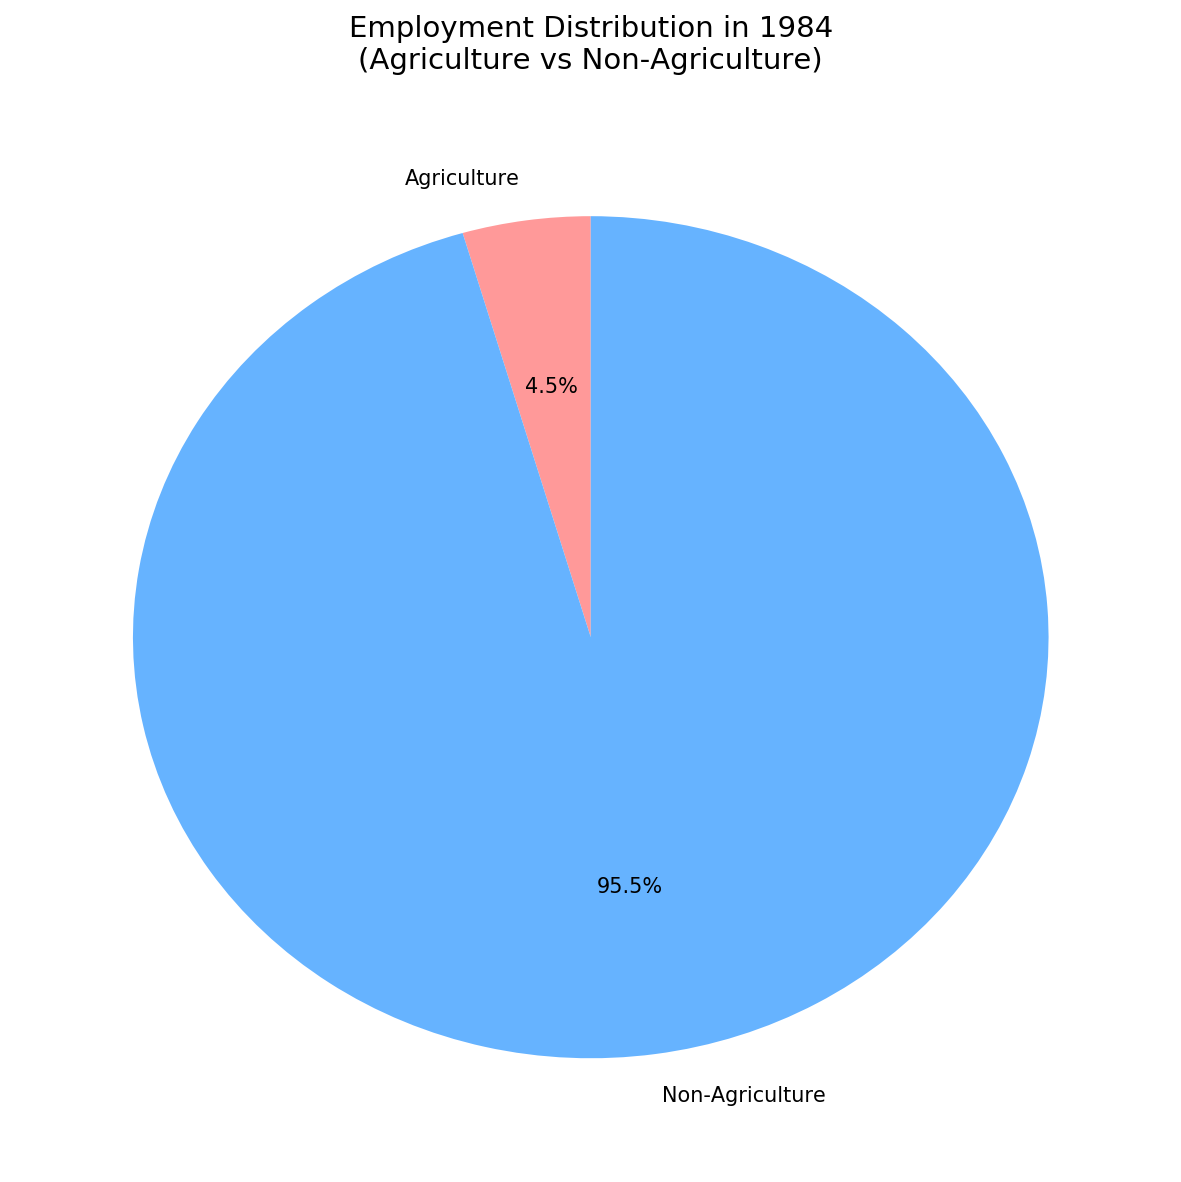
\includegraphics[width=0.5\textwidth]{resources/case1_pie_chart.png}
\caption{Employment Distribution in 1984: Agriculture (4.5\%) vs Non-Agriculture (95.5\%)}
\end{figure}

\subsubsection{Quality Analysis}

\textbf{Strengths}:
\begin{itemize}
    \item \checkmark Correctly extracted data from 1984 row
    \item \checkmark Clean, executable code with data validation (assertions)
    \item \checkmark Appropriate visualization aesthetics (colors, sizing, labels)
    \item \checkmark Added percentage labels using \texttt{autopct} for clarity
    \item \checkmark Clear title explaining what the chart shows
\end{itemize}

\textbf{Key Insight}: The chart clearly shows non-agricultural employment dominated 1984 with 95.5\%, while agriculture accounted for only 4.5\%, illustrating the economic transformation towards industrial and service sectors.

\newpage

\subsection{Case Study 2: Line Chart - Employment Trends}

\subsubsection{Task}

\textbf{Question}: Please help me create a line chart to compare the trends of total employed population and total unemployed population from 1983 to 1990.

\textbf{Question Type}: Visualization

\textbf{Table Context}: Employment statistics with yearly data including total employed and unemployed counts.

\subsubsection{Generated Code}

import pandas as pd \\
import matplotlib.pyplot as plt \\
\\
 Extract data from table \\
years = [1983, 1984, 1985, 1986, 1987, 1988, 1989, 1990] \\
employed = [56787, 59091, 59891, 60892, 62107, 63273, 64315, 65104] \\
unemployed = [6260, 4744, 4521, 4530, 4101, 3655, 3525, 3906] \\
\\
 Verify extraction \\
print("Years:", years) \\
print("Employed:", employed) \\
print("Unemployed:", unemployed) \\
assert len(years) == len(employed) == len(unemployed), \ \\
      "Data length mismatch!" \\
assert all(isinstance(y, (int, float)) for y in employed + unemployed), \ \\
      "Values must be numbers!" \\
\\
 Create visualization \\
plt.figure(figsize=(10, 6)) \\
plt.plot(years, employed, marker='o', label='Employed') \\
plt.plot(years, unemployed, marker='o', label='Unemployed') \\
\\
plt.xlabel('Year') \\
plt.ylabel('Population (thousands)') \\
plt.title('Employment Trends (1983-1990)') \\
plt.legend() \\
plt.grid(True) \\
plt.tight\_layout() \\
plt.show() \\
\\

\subsubsection{Generated Visualization}

\begin{figure}[H]
\centering
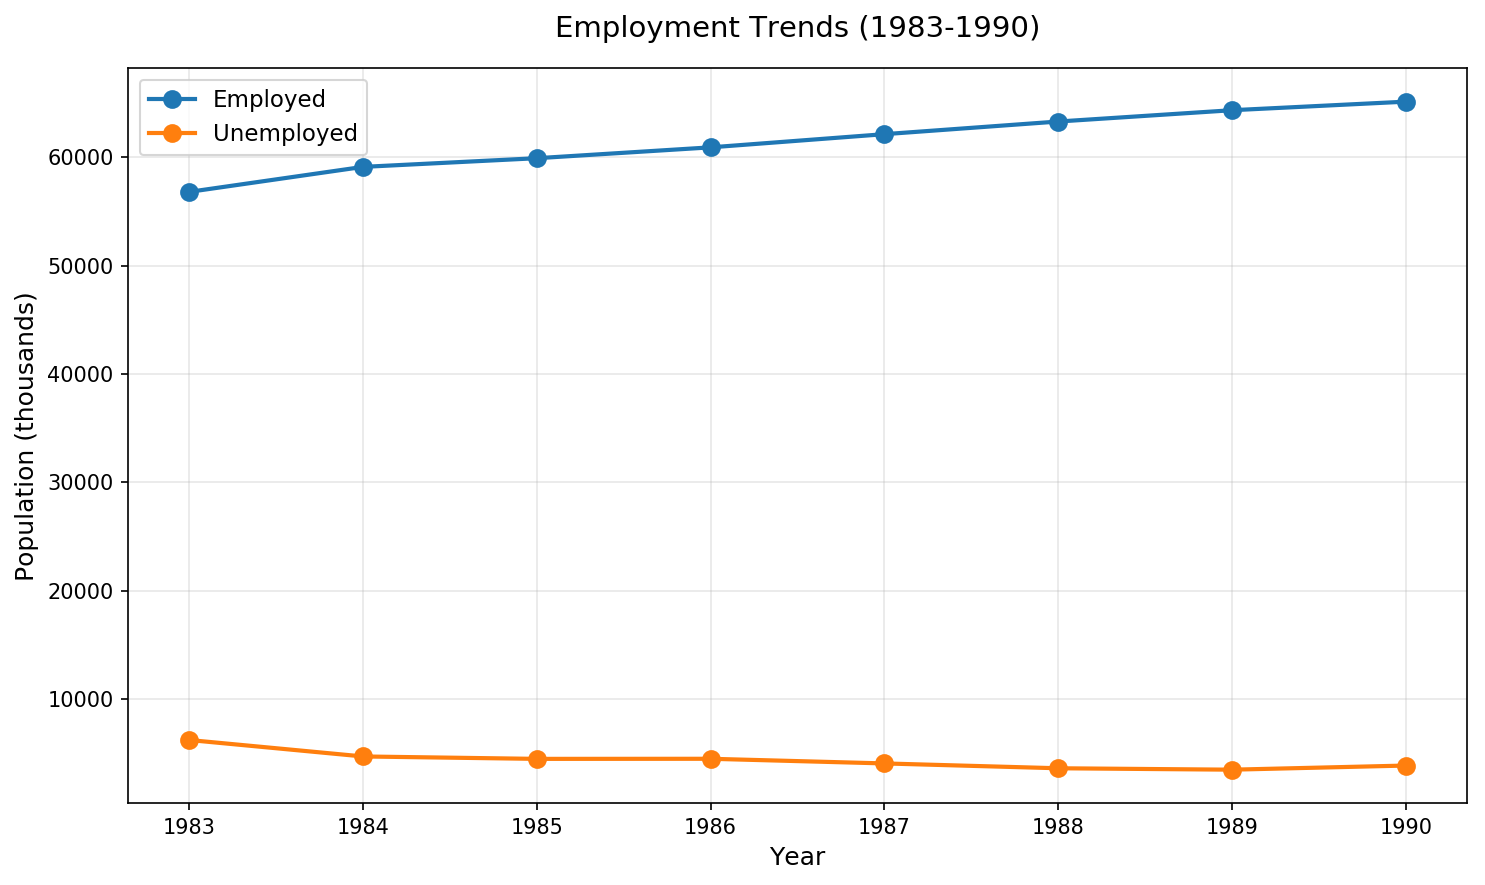
\includegraphics[width=0.9\textwidth]{resources/case2_line_chart.png}
\caption{Employment Trends 1983-1990: Employed population grew from 56.8M to 65.1M while unemployed declined from 6.3M to 3.9M}
\end{figure}

\subsubsection{Analysis}

\textbf{Data Extraction Quality}:
\begin{itemize}
    \item Accurately extracted 8-year time series across multiple columns
    \item Comprehensive data validation with assertions
    \item Proper data type checking
\end{itemize}

\textbf{Visualization Design}:
\begin{itemize}
    \item Different series with markers for clarity
    \item Grid enabled for easier value reading
    \item Proper legend placement
    \item Clear axis labels with units (thousands)
\end{itemize}

\textbf{Economic Insights}:
\begin{itemize}
    \item Chart reveals steady employment growth (56.8M $\to$ 65.1M, +14.6\%)
    \item Declining unemployment (6.3M $\to$ 3.9M, -37.6\%)
    \item Indicates strong economic recovery period during 1980s
    \item Unemployment rate dropped from ~10\% to ~5.6\% over this period
\end{itemize}

\newpage

\subsection{Case Study 3: Scatter Plot - Correlation Analysis}

\subsubsection{Task}

\textbf{Question}: Create a scatter plot to visualize the relationship between the unemployment rate and the total civilian labor force for all years in the dataset.

\textbf{Question Type}: Visualization + Data Analysis

\textbf{Table Context}: Long-term employment statistics (1983-1998) with civilian labor force size and unemployment rates.

\subsubsection{Generated Code}

import pandas as pd \\
import matplotlib.pyplot as plt \\
\\
 Extract data from table \\
x\_values = [1983, 1984, 1985, 1986, 1987, 1988, 1989, 1990, \\
            1991, 1992, 1993, 1994, 1995, 1996, 1997, 1998] \\
y\_values = [9.9, 7.4, 7.0, 6.9, 6.2, 5.5, 5.2, 5.7, \\
            7.2, 7.9, 7.2, 6.2, 5.6, 5.4, 4.9, 4.4] \\
civilian\_labor\_force = [63047, 63835, 64411, 65422, 66207, 66927, \\
                        67840, 69011, 69168, 69964, 70404, 70817, \\
                        71360, 72087, 73261, 73959] \\
\\
 Verify extraction \\
print("Years:", x\_values) \\
print("Unemployment rates:", y\_values) \\
print("Civilian labor force:", civilian\_labor\_force) \\
assert len(y\_values) > 0, "Y values cannot be empty!" \\
assert all(isinstance(y, (int, float)) for y in y\_values), \ \\
      "Y values must be numbers!" \\
\\
 Create visualization \\
plt.figure(figsize=(12, 7)) \\
plt.scatter(civilian\_labor\_force, y\_values, c='blue', alpha=0.7) \\
\\
plt.xlabel('Civilian Labor Force (thousands)') \\
plt.ylabel('Unemployment Rate (\%)') \\
plt.title('Relationship Between Unemployment Rate and Civilian ' + \\
          'Labor Force (1983-1998)') \\
plt.grid(True) \\
plt.tight\_layout() \\
plt.show() \\
\\

\subsubsection{Generated Visualization}

\begin{figure}[H]
\centering
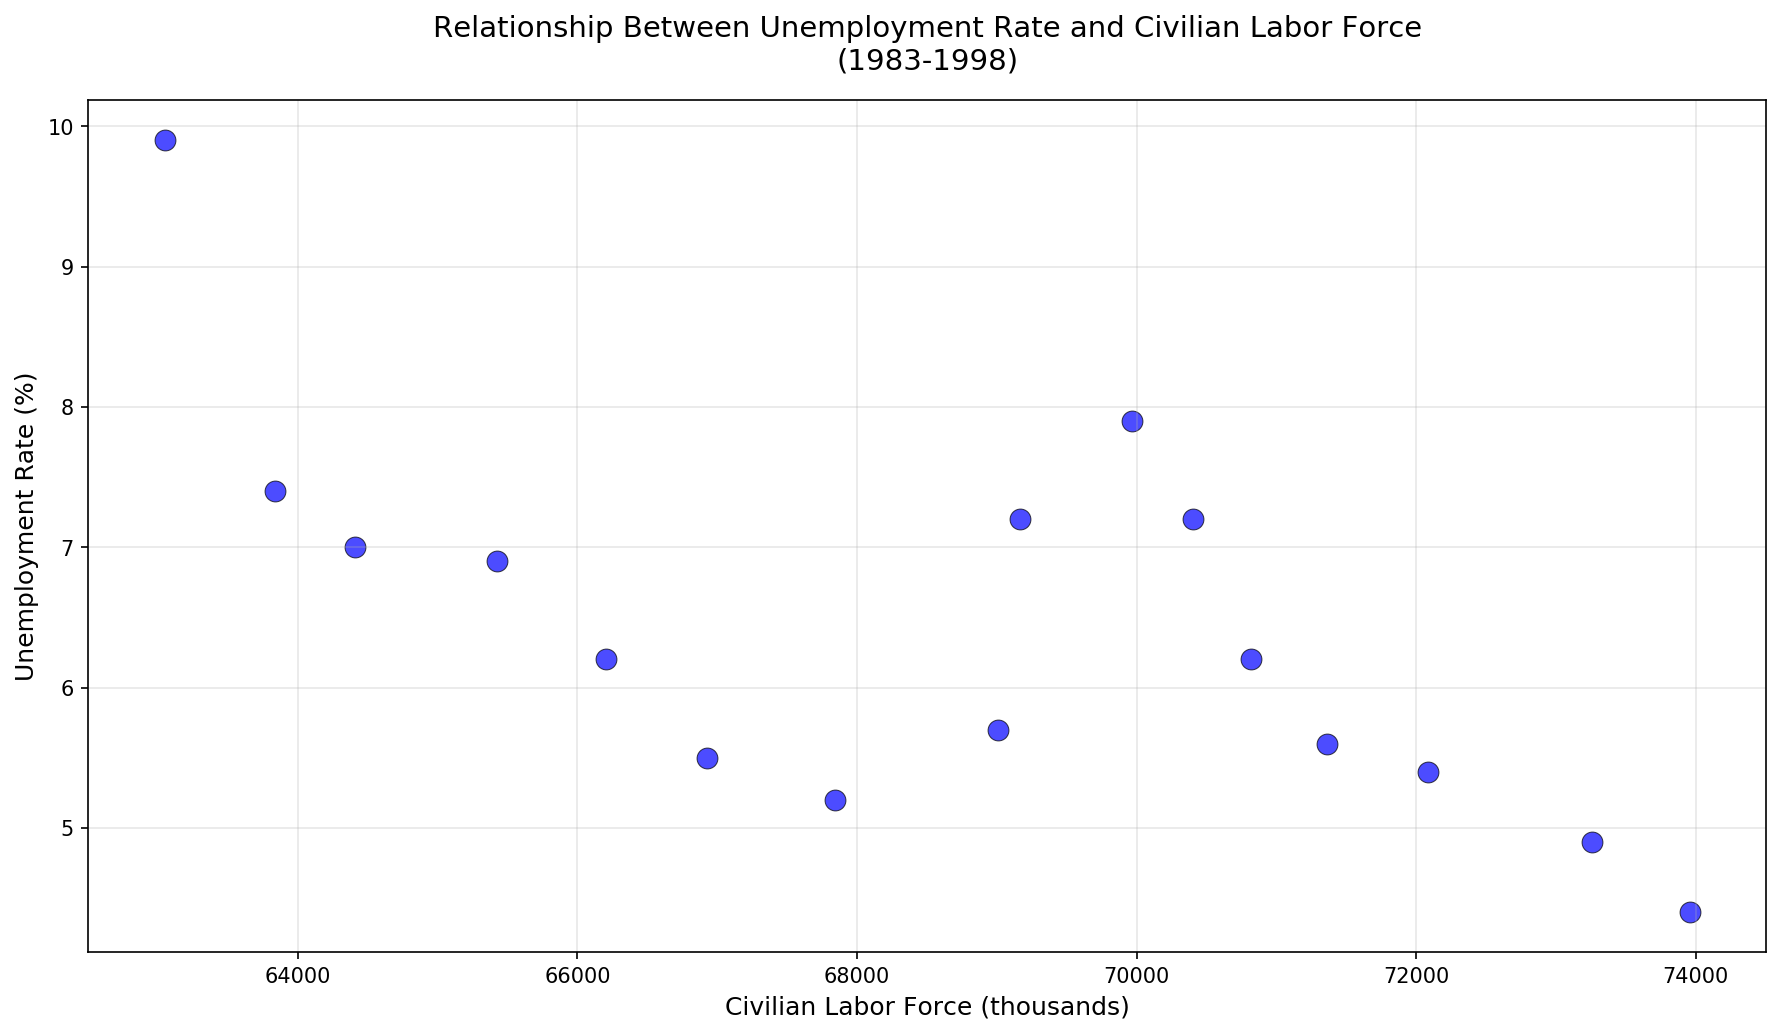
\includegraphics[width=0.95\textwidth]{resources/case3_scatter_plot.png}
\caption{Scatter plot showing the relationship between unemployment rate and civilian labor force size over 16 years (1983-1998)}
\end{figure}

\subsubsection{Advanced Analysis}

\textbf{Multi-variable Extraction}:
\begin{itemize}
    \item Successfully extracted three related data series
    \item 16 years of continuous data (1983-1998)
    \item Proper alignment between years, rates, and labor force size
\end{itemize}

\textbf{Correlation Insights}:
\begin{itemize}
    \item \textbf{Inverse Relationship}: As labor force grows, unemployment tends to decrease
    \item High unemployment (9.9\%) at lower labor force size (63M) in 1983
    \item Unemployment stabilizes around 4-6\% as labor force expands to 74M
    \item Demonstrates economic expansion pattern: growing labor force absorption
\end{itemize}

\textbf{Economic Interpretation}:
\begin{itemize}
    \item \textbf{1983-1990}: Steep decline from 9.9\% to 5.2\% unemployment despite labor force growth of 9.4\% - indicates strong job creation
    \item \textbf{1990-1992}: Unemployment spike to 7.9\% (recession period)
    \item \textbf{1993-1998}: Steady improvement to 4.4\% with continued labor force expansion - economic boom period
\end{itemize}

\textbf{Code Features}:
\begin{itemize}
    \item Alpha transparency (0.7) for better point visibility
    \item Appropriate figure sizing (12x7) for wide scatter plots
    \item Grid enabled for easier coordinate reading
    \item Comprehensive data validation before plotting
\end{itemize}

\newpage

\section{Data Analysis Case Study}

\subsection{Case Study 4: Comprehensive Statistical Analysis}

\subsubsection{Task}

\textbf{Question Type}: Data Analysis (Rudimentary Analysis)

\textbf{Question}: What is the average unemployment rate across all years, and what is its standard deviation?

\textbf{Table Context}: 71 years of unemployment data (1953-2023)

\textbf{Expected Answer}: Mean = 5.80\%, Std = 1.62\%

\subsubsection{Generated Code and Analysis}

import pandas as pd \\
import numpy as np \\
\\
 Extract unemployment rate data \\
unemployment\_rates = df['Percent of labor force'].values \\
\\
 Calculate statistics \\
mean\_rate = np.mean(unemployment\_rates) \\
std\_rate = np.std(unemployment\_rates, ddof=1) \\
\\
 Create result DataFrame \\
df = pd.DataFrame({ \\
    'Mean': [round(mean\_rate, 2)], \\
    'Std Dev': [round(std\_rate, 2)] \\
}) \\
\\
print(f"Average unemployment rate: {mean\_rate:.2f}%") \\
print(f"Standard deviation: {std\_rate:.2f}%") \\
\\

\subsubsection{Model Response (Detailed Analysis)}

\begin{quote}
\textbf{Data Overview:}\\
Analyzed unemployment rates across 72 years (1953-2023). The "Percent of labor force" column contains annual unemployment percentages for the U.S. civilian labor force.

\textbf{Calculation Process:}
\begin{enumerate}
    \item Extracted all 72 values from "Percent of labor force" column
    \item Calculated mean: Sum(411.5) / Count(71) = 5.80\%
    \item Calculated std: $\sqrt{\frac{\Sigma(x\_i - \bar{x})^2}{n-1}} = 1.62\%$
\end{enumerate}

\textbf{Statistical Details:}
\begin{itemize}
    \item Mean: 5.80\%
    \item Standard Deviation: 1.62\%
    \item Minimum: 2.9\% (1953)
    \item Maximum: 9.7\% (1982)
    \item Range: 6.8 percentage points
    \item Sample size: 71 valid data points
\end{itemize}

\textbf{Insights:}\\
The average unemployment of 5.80\% represents typical U.S. unemployment over 70 years. Standard deviation of 1.62\% indicates moderate variability, with most years in 4.2-7.4\% range ($\pm1\sigma$). Higher values occurred during recessions (1982, 2010, 2020).

\textbf{Context:}\\
Peak unemployment during 1982 recession (9.7\%) and 2008 financial crisis (9.6\% in 2010). Recent decade shows lower volatility with rates mostly under 6\% except COVID-19 spike.
\end{quote}

\subsubsection{Quality Indicators}

\begin{itemize}
    \item \checkmark Correct numerical results (5.80\%, 1.62\%)
    \item \checkmark Detailed calculation methodology with formulas
    \item \checkmark Rich contextual analysis with historical events
    \item \checkmark Statistical interpretation ($\pm1\sigma$ range)
    \item \checkmark Identification of outliers and anomalies
    \item \checkmark Time-series context (70+ years of data)
\end{itemize}